% Created by tikzDevice version 0.12.4 on 2023-07-16 15:10:06
% !TEX encoding = UTF-8 Unicode
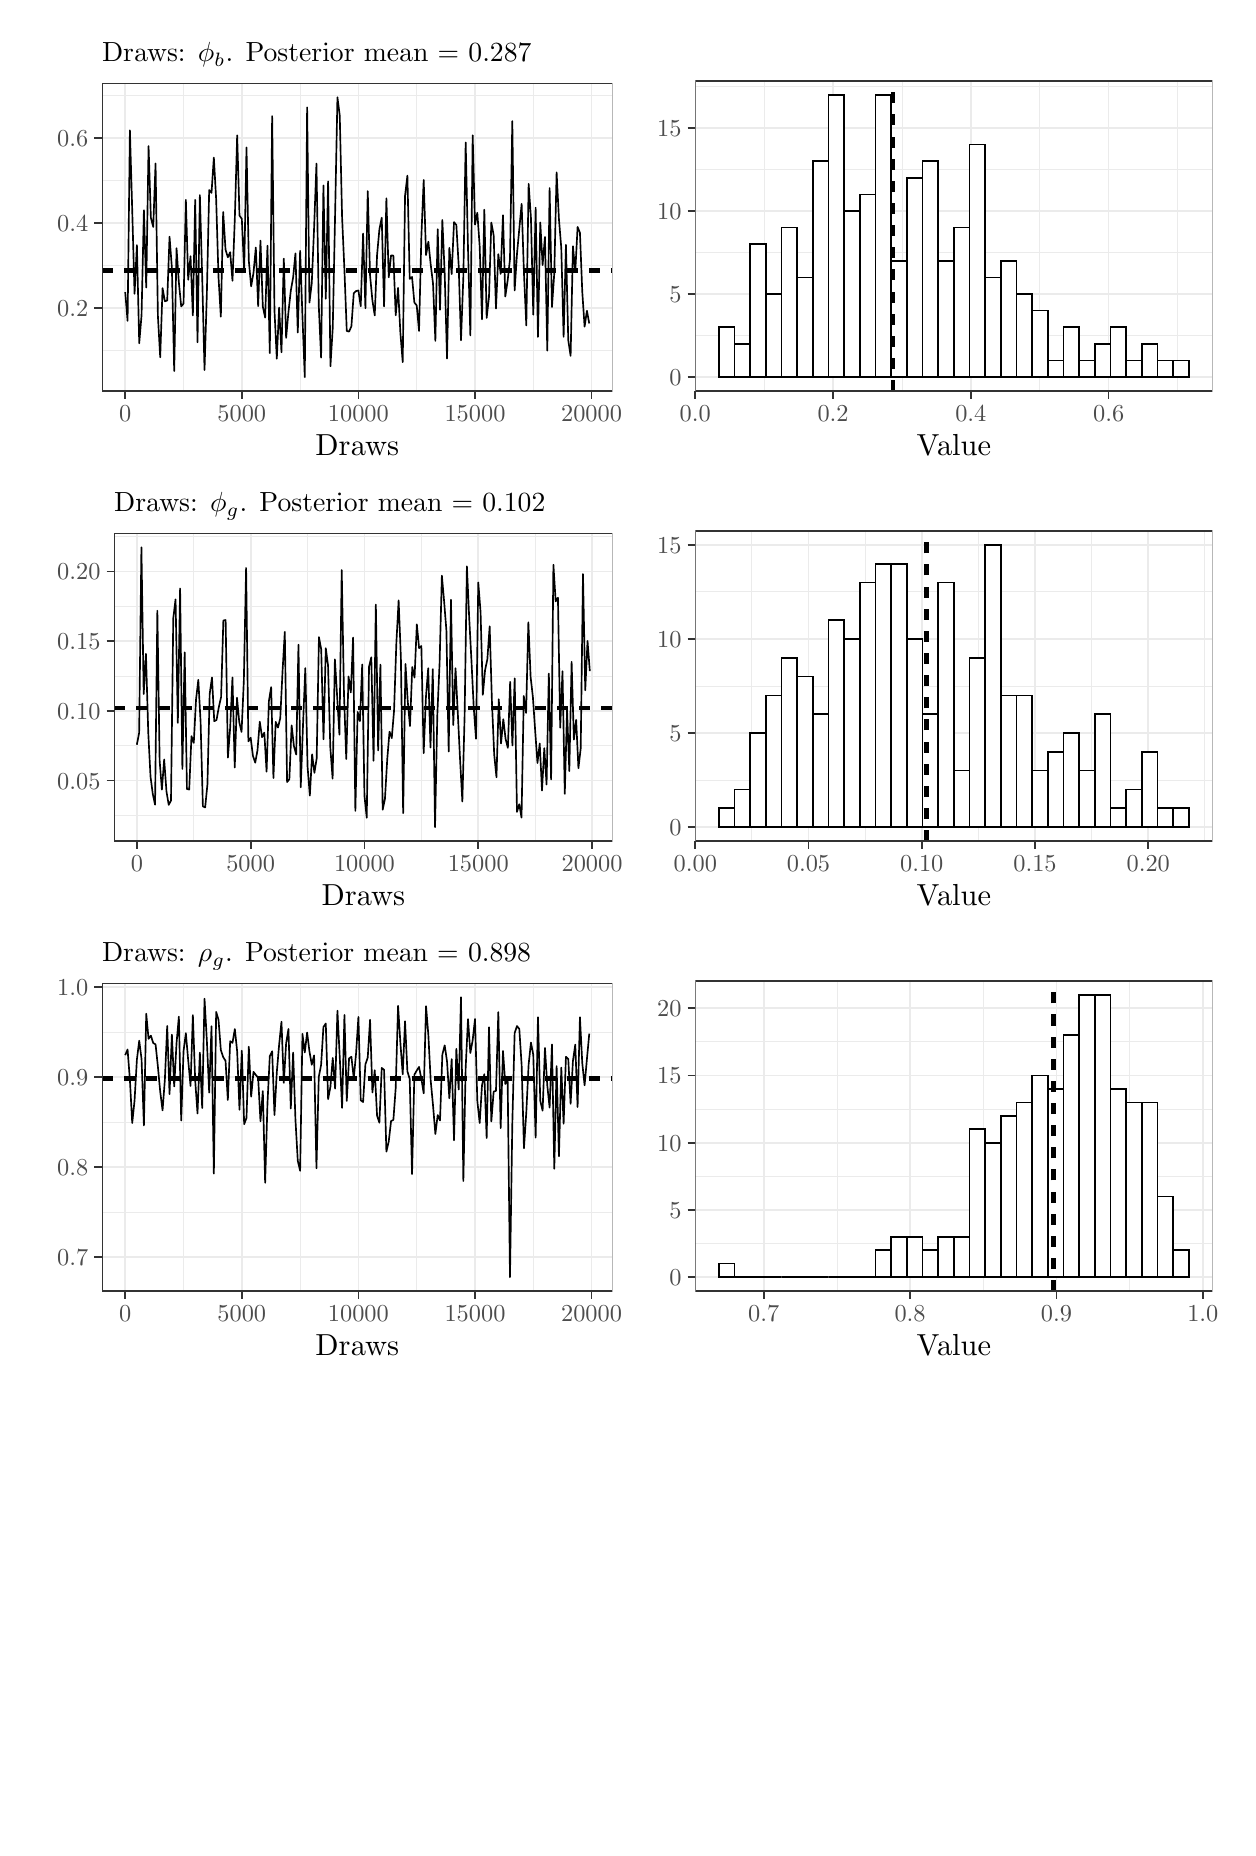
\begin{tikzpicture}[x=1pt,y=1pt]
\definecolor{fillColor}{RGB}{255,255,255}
\path[use as bounding box,fill=fillColor,fill opacity=0.00] (0,0) rectangle (433.62,650.43);
\begin{scope}
\path[clip] (  0.00,487.82) rectangle (216.81,650.43);
\definecolor{drawColor}{RGB}{255,255,255}
\definecolor{fillColor}{RGB}{255,255,255}

\path[draw=drawColor,line width= 0.6pt,line join=round,line cap=round,fill=fillColor] (  0.00,487.82) rectangle (216.81,650.43);
\end{scope}
\begin{scope}
\path[clip] ( 26.87,519.08) rectangle (211.31,630.33);
\definecolor{fillColor}{RGB}{255,255,255}

\path[fill=fillColor] ( 26.87,519.08) rectangle (211.31,630.33);
\definecolor{drawColor}{gray}{0.92}

\path[draw=drawColor,line width= 0.3pt,line join=round] ( 26.87,533.91) --
	(211.31,533.91);

\path[draw=drawColor,line width= 0.3pt,line join=round] ( 26.87,564.58) --
	(211.31,564.58);

\path[draw=drawColor,line width= 0.3pt,line join=round] ( 26.87,595.24) --
	(211.31,595.24);

\path[draw=drawColor,line width= 0.3pt,line join=round] ( 26.87,625.91) --
	(211.31,625.91);

\path[draw=drawColor,line width= 0.3pt,line join=round] ( 56.32,519.08) --
	( 56.32,630.33);

\path[draw=drawColor,line width= 0.3pt,line join=round] ( 98.45,519.08) --
	( 98.45,630.33);

\path[draw=drawColor,line width= 0.3pt,line join=round] (140.58,519.08) --
	(140.58,630.33);

\path[draw=drawColor,line width= 0.3pt,line join=round] (182.70,519.08) --
	(182.70,630.33);

\path[draw=drawColor,line width= 0.6pt,line join=round] ( 26.87,549.24) --
	(211.31,549.24);

\path[draw=drawColor,line width= 0.6pt,line join=round] ( 26.87,579.91) --
	(211.31,579.91);

\path[draw=drawColor,line width= 0.6pt,line join=round] ( 26.87,610.57) --
	(211.31,610.57);

\path[draw=drawColor,line width= 0.6pt,line join=round] ( 35.25,519.08) --
	( 35.25,630.33);

\path[draw=drawColor,line width= 0.6pt,line join=round] ( 77.38,519.08) --
	( 77.38,630.33);

\path[draw=drawColor,line width= 0.6pt,line join=round] (119.51,519.08) --
	(119.51,630.33);

\path[draw=drawColor,line width= 0.6pt,line join=round] (161.64,519.08) --
	(161.64,630.33);

\path[draw=drawColor,line width= 0.6pt,line join=round] (203.77,519.08) --
	(203.77,630.33);
\definecolor{drawColor}{RGB}{0,0,0}

\path[draw=drawColor,line width= 0.6pt,line join=round] ( 35.25,554.89) --
	( 36.10,544.46) --
	( 36.94,613.34) --
	( 37.78,584.41) --
	( 38.62,554.24) --
	( 39.47,571.83) --
	( 40.31,536.40) --
	( 41.15,546.52) --
	( 42.00,584.47) --
	( 42.84,556.50) --
	( 43.68,607.65) --
	( 44.52,581.70) --
	( 45.37,578.42) --
	( 46.21,601.36) --
	( 47.05,546.38) --
	( 47.89,531.33) --
	( 48.74,556.32) --
	( 49.58,551.56) --
	( 50.42,551.82) --
	( 51.26,574.91) --
	( 52.11,563.68) --
	( 52.95,526.34) --
	( 53.79,570.75) --
	( 54.63,558.40) --
	( 55.48,549.69) --
	( 56.32,550.70) --
	( 57.16,588.19) --
	( 58.00,559.33) --
	( 58.85,567.82) --
	( 59.69,546.42) --
	( 60.53,588.21) --
	( 61.37,536.72) --
	( 62.22,589.96) --
	( 63.06,560.52) --
	( 63.90,526.68) --
	( 64.74,554.09) --
	( 65.59,591.75) --
	( 66.43,590.71) --
	( 67.27,603.48) --
	( 68.11,588.40) --
	( 68.96,560.18) --
	( 69.80,545.97) --
	( 70.64,583.82) --
	( 71.49,570.24) --
	( 72.33,567.45) --
	( 73.17,569.30) --
	( 74.01,558.98) --
	( 74.86,581.65) --
	( 75.70,611.54) --
	( 76.54,582.51) --
	( 77.38,581.35) --
	( 78.23,562.72) --
	( 79.07,607.10) --
	( 79.91,566.22) --
	( 80.75,556.95) --
	( 81.60,561.82) --
	( 82.44,570.98) --
	( 83.28,549.78) --
	( 84.12,573.48) --
	( 84.97,549.65) --
	( 85.81,545.66) --
	( 86.65,571.60) --
	( 87.49,532.81) --
	( 88.34,618.46) --
	( 89.18,548.27) --
	( 90.02,530.80) --
	( 90.86,549.31) --
	( 91.71,533.12) --
	( 92.55,566.97) --
	( 93.39,538.35) --
	( 94.23,547.67) --
	( 95.08,555.37) --
	( 95.92,560.15) --
	( 96.76,568.88) --
	( 97.60,540.23) --
	( 98.45,569.77) --
	( 99.29,546.05) --
	(100.13,524.13) --
	(100.98,621.60) --
	(101.82,551.10) --
	(102.66,558.15) --
	(103.50,578.07) --
	(104.35,601.32) --
	(105.19,549.97) --
	(106.03,531.18) --
	(106.87,593.42) --
	(107.72,552.45) --
	(108.56,594.86) --
	(109.40,528.08) --
	(110.24,541.97) --
	(111.09,582.95) --
	(111.93,625.28) --
	(112.77,618.64) --
	(113.61,582.07) --
	(114.46,562.80) --
	(115.30,540.85) --
	(116.14,540.59) --
	(116.98,542.53) --
	(117.83,554.49) --
	(118.67,555.24) --
	(119.51,555.45) --
	(120.35,549.78) --
	(121.20,576.02) --
	(122.04,549.02) --
	(122.88,591.37) --
	(123.72,560.87) --
	(124.57,551.83) --
	(125.41,546.45) --
	(126.25,568.22) --
	(127.09,577.51) --
	(127.94,581.77) --
	(128.78,549.71) --
	(129.62,588.78) --
	(130.47,560.20) --
	(131.31,568.13) --
	(132.15,568.06) --
	(132.99,546.48) --
	(133.84,556.38) --
	(134.68,540.08) --
	(135.52,529.56) --
	(136.36,589.66) --
	(137.21,596.95) --
	(138.05,559.65) --
	(138.89,560.35) --
	(139.73,551.11) --
	(140.58,550.05) --
	(141.42,540.84) --
	(142.26,574.98) --
	(143.10,595.38) --
	(143.95,568.26) --
	(144.79,573.08) --
	(145.63,564.86) --
	(146.47,557.96) --
	(147.32,537.25) --
	(148.16,577.58) --
	(149.00,548.49) --
	(149.84,580.94) --
	(150.69,561.56) --
	(151.53,530.86) --
	(152.37,570.88) --
	(153.21,561.38) --
	(154.06,580.15) --
	(154.90,579.12) --
	(155.74,564.54) --
	(156.58,537.45) --
	(157.43,560.38) --
	(158.27,608.95) --
	(159.11,570.66) --
	(159.96,539.20) --
	(160.80,611.54) --
	(161.64,579.26) --
	(162.48,583.53) --
	(163.33,571.41) --
	(164.17,545.04) --
	(165.01,584.63) --
	(165.85,545.52) --
	(166.70,553.18) --
	(167.54,580.00) --
	(168.38,575.46) --
	(169.22,548.94) --
	(170.07,568.58) --
	(170.91,561.43) --
	(171.75,582.68) --
	(172.59,553.29) --
	(173.44,559.06) --
	(174.28,566.78) --
	(175.12,616.66) --
	(175.96,555.44) --
	(176.81,568.65) --
	(177.65,577.75) --
	(178.49,586.75) --
	(179.33,561.77) --
	(180.18,542.82) --
	(181.02,594.00) --
	(181.86,581.63) --
	(182.70,546.71) --
	(183.55,585.37) --
	(184.39,538.67) --
	(185.23,580.04) --
	(186.07,564.65) --
	(186.92,574.81) --
	(187.76,533.72) --
	(188.60,592.46) --
	(189.45,549.48) --
	(190.29,561.70) --
	(191.13,598.12) --
	(191.97,581.28) --
	(192.82,570.79) --
	(193.66,538.72) --
	(194.50,571.96) --
	(195.34,537.48) --
	(196.19,531.82) --
	(197.03,571.47) --
	(197.87,562.18) --
	(198.71,578.41) --
	(199.56,576.33) --
	(200.40,555.04) --
	(201.24,542.37) --
	(202.08,548.13) --
	(202.93,543.53);

\path[draw=drawColor,line width= 1.7pt,dash pattern=on 4pt off 4pt ,line join=round] ( 26.87,562.58) -- (211.31,562.58);
\definecolor{drawColor}{gray}{0.20}

\path[draw=drawColor,line width= 0.6pt,line join=round,line cap=round] ( 26.87,519.08) rectangle (211.31,630.33);
\end{scope}
\begin{scope}
\path[clip] (  0.00,  0.00) rectangle (433.62,650.43);
\definecolor{drawColor}{gray}{0.30}

\node[text=drawColor,anchor=base east,inner sep=0pt, outer sep=0pt, scale=  0.88] at ( 21.92,546.21) {0.2};

\node[text=drawColor,anchor=base east,inner sep=0pt, outer sep=0pt, scale=  0.88] at ( 21.92,576.88) {0.4};

\node[text=drawColor,anchor=base east,inner sep=0pt, outer sep=0pt, scale=  0.88] at ( 21.92,607.54) {0.6};
\end{scope}
\begin{scope}
\path[clip] (  0.00,  0.00) rectangle (433.62,650.43);
\definecolor{drawColor}{gray}{0.20}

\path[draw=drawColor,line width= 0.6pt,line join=round] ( 24.12,549.24) --
	( 26.87,549.24);

\path[draw=drawColor,line width= 0.6pt,line join=round] ( 24.12,579.91) --
	( 26.87,579.91);

\path[draw=drawColor,line width= 0.6pt,line join=round] ( 24.12,610.57) --
	( 26.87,610.57);
\end{scope}
\begin{scope}
\path[clip] (  0.00,  0.00) rectangle (433.62,650.43);
\definecolor{drawColor}{gray}{0.20}

\path[draw=drawColor,line width= 0.6pt,line join=round] ( 35.25,516.33) --
	( 35.25,519.08);

\path[draw=drawColor,line width= 0.6pt,line join=round] ( 77.38,516.33) --
	( 77.38,519.08);

\path[draw=drawColor,line width= 0.6pt,line join=round] (119.51,516.33) --
	(119.51,519.08);

\path[draw=drawColor,line width= 0.6pt,line join=round] (161.64,516.33) --
	(161.64,519.08);

\path[draw=drawColor,line width= 0.6pt,line join=round] (203.77,516.33) --
	(203.77,519.08);
\end{scope}
\begin{scope}
\path[clip] (  0.00,  0.00) rectangle (433.62,650.43);
\definecolor{drawColor}{gray}{0.30}

\node[text=drawColor,anchor=base,inner sep=0pt, outer sep=0pt, scale=  0.88] at ( 35.25,508.06) {0};

\node[text=drawColor,anchor=base,inner sep=0pt, outer sep=0pt, scale=  0.88] at ( 77.38,508.06) {5000};

\node[text=drawColor,anchor=base,inner sep=0pt, outer sep=0pt, scale=  0.88] at (119.51,508.06) {10000};

\node[text=drawColor,anchor=base,inner sep=0pt, outer sep=0pt, scale=  0.88] at (161.64,508.06) {15000};

\node[text=drawColor,anchor=base,inner sep=0pt, outer sep=0pt, scale=  0.88] at (203.77,508.06) {20000};
\end{scope}
\begin{scope}
\path[clip] (  0.00,  0.00) rectangle (433.62,650.43);
\definecolor{drawColor}{RGB}{0,0,0}

\node[text=drawColor,anchor=base,inner sep=0pt, outer sep=0pt, scale=  1.10] at (119.09,495.75) {Draws};
\end{scope}
\begin{scope}
\path[clip] (  0.00,  0.00) rectangle (433.62,650.43);
\definecolor{drawColor}{RGB}{0,0,0}

\node[text=drawColor,anchor=base west,inner sep=0pt, outer sep=0pt, scale=  1.00] at ( 26.87,638.04) {Draws: $\phi_b$. Posterior mean = 0.287};
\end{scope}
\begin{scope}
\path[clip] (216.81,487.82) rectangle (433.62,650.43);
\definecolor{drawColor}{RGB}{255,255,255}
\definecolor{fillColor}{RGB}{255,255,255}

\path[draw=drawColor,line width= 0.6pt,line join=round,line cap=round,fill=fillColor] (216.81,487.82) rectangle (433.62,650.43);
\end{scope}
\begin{scope}
\path[clip] (241.24,519.08) rectangle (428.12,631.24);
\definecolor{fillColor}{RGB}{255,255,255}

\path[fill=fillColor] (241.24,519.08) rectangle (428.12,631.24);
\definecolor{drawColor}{gray}{0.92}

\path[draw=drawColor,line width= 0.3pt,line join=round] (241.24,539.17) --
	(428.12,539.17);

\path[draw=drawColor,line width= 0.3pt,line join=round] (241.24,569.16) --
	(428.12,569.16);

\path[draw=drawColor,line width= 0.3pt,line join=round] (241.24,599.15) --
	(428.12,599.15);

\path[draw=drawColor,line width= 0.3pt,line join=round] (241.24,629.14) --
	(428.12,629.14);

\path[draw=drawColor,line width= 0.3pt,line join=round] (266.13,519.08) --
	(266.13,631.24);

\path[draw=drawColor,line width= 0.3pt,line join=round] (315.92,519.08) --
	(315.92,631.24);

\path[draw=drawColor,line width= 0.3pt,line join=round] (365.72,519.08) --
	(365.72,631.24);

\path[draw=drawColor,line width= 0.3pt,line join=round] (415.51,519.08) --
	(415.51,631.24);

\path[draw=drawColor,line width= 0.6pt,line join=round] (241.24,524.17) --
	(428.12,524.17);

\path[draw=drawColor,line width= 0.6pt,line join=round] (241.24,554.17) --
	(428.12,554.17);

\path[draw=drawColor,line width= 0.6pt,line join=round] (241.24,584.16) --
	(428.12,584.16);

\path[draw=drawColor,line width= 0.6pt,line join=round] (241.24,614.15) --
	(428.12,614.15);

\path[draw=drawColor,line width= 0.6pt,line join=round] (241.24,519.08) --
	(241.24,631.24);

\path[draw=drawColor,line width= 0.6pt,line join=round] (291.03,519.08) --
	(291.03,631.24);

\path[draw=drawColor,line width= 0.6pt,line join=round] (340.82,519.08) --
	(340.82,631.24);

\path[draw=drawColor,line width= 0.6pt,line join=round] (390.61,519.08) --
	(390.61,631.24);
\definecolor{drawColor}{RGB}{0,0,0}

\path[draw=drawColor,line width= 0.6pt,fill=fillColor] (249.73,524.17) rectangle (255.39,542.17);

\path[draw=drawColor,line width= 0.6pt,fill=fillColor] (255.39,524.17) rectangle (261.06,536.17);

\path[draw=drawColor,line width= 0.6pt,fill=fillColor] (261.06,524.17) rectangle (266.72,572.16);

\path[draw=drawColor,line width= 0.6pt,fill=fillColor] (266.72,524.17) rectangle (272.38,554.17);

\path[draw=drawColor,line width= 0.6pt,fill=fillColor] (272.38,524.17) rectangle (278.05,578.16);

\path[draw=drawColor,line width= 0.6pt,fill=fillColor] (278.05,524.17) rectangle (283.71,560.16);

\path[draw=drawColor,line width= 0.6pt,fill=fillColor] (283.71,524.17) rectangle (289.37,602.15);

\path[draw=drawColor,line width= 0.6pt,fill=fillColor] (289.37,524.17) rectangle (295.04,626.15);

\path[draw=drawColor,line width= 0.6pt,fill=fillColor] (295.04,524.17) rectangle (300.70,584.16);

\path[draw=drawColor,line width= 0.6pt,fill=fillColor] (300.70,524.17) rectangle (306.36,590.16);

\path[draw=drawColor,line width= 0.6pt,fill=fillColor] (306.36,524.17) rectangle (312.03,626.15);

\path[draw=drawColor,line width= 0.6pt,fill=fillColor] (312.03,524.17) rectangle (317.69,566.16);

\path[draw=drawColor,line width= 0.6pt,fill=fillColor] (317.69,524.17) rectangle (323.35,596.15);

\path[draw=drawColor,line width= 0.6pt,fill=fillColor] (323.35,524.17) rectangle (329.02,602.15);

\path[draw=drawColor,line width= 0.6pt,fill=fillColor] (329.02,524.17) rectangle (334.68,566.16);

\path[draw=drawColor,line width= 0.6pt,fill=fillColor] (334.68,524.17) rectangle (340.34,578.16);

\path[draw=drawColor,line width= 0.6pt,fill=fillColor] (340.34,524.17) rectangle (346.00,608.15);

\path[draw=drawColor,line width= 0.6pt,fill=fillColor] (346.00,524.17) rectangle (351.67,560.16);

\path[draw=drawColor,line width= 0.6pt,fill=fillColor] (351.67,524.17) rectangle (357.33,566.16);

\path[draw=drawColor,line width= 0.6pt,fill=fillColor] (357.33,524.17) rectangle (362.99,554.17);

\path[draw=drawColor,line width= 0.6pt,fill=fillColor] (362.99,524.17) rectangle (368.66,548.17);

\path[draw=drawColor,line width= 0.6pt,fill=fillColor] (368.66,524.17) rectangle (374.32,530.17);

\path[draw=drawColor,line width= 0.6pt,fill=fillColor] (374.32,524.17) rectangle (379.98,542.17);

\path[draw=drawColor,line width= 0.6pt,fill=fillColor] (379.98,524.17) rectangle (385.65,530.17);

\path[draw=drawColor,line width= 0.6pt,fill=fillColor] (385.65,524.17) rectangle (391.31,536.17);

\path[draw=drawColor,line width= 0.6pt,fill=fillColor] (391.31,524.17) rectangle (396.97,542.17);

\path[draw=drawColor,line width= 0.6pt,fill=fillColor] (396.97,524.17) rectangle (402.64,530.17);

\path[draw=drawColor,line width= 0.6pt,fill=fillColor] (402.64,524.17) rectangle (408.30,536.17);

\path[draw=drawColor,line width= 0.6pt,fill=fillColor] (408.30,524.17) rectangle (413.96,530.17);

\path[draw=drawColor,line width= 0.6pt,fill=fillColor] (413.96,524.17) rectangle (419.63,530.17);

\path[draw=drawColor,line width= 1.7pt,dash pattern=on 4pt off 4pt ,line join=round] (312.69,519.08) -- (312.69,631.24);
\definecolor{drawColor}{gray}{0.20}

\path[draw=drawColor,line width= 0.6pt,line join=round,line cap=round] (241.24,519.08) rectangle (428.12,631.24);
\end{scope}
\begin{scope}
\path[clip] (  0.00,  0.00) rectangle (433.62,650.43);
\definecolor{drawColor}{gray}{0.30}

\node[text=drawColor,anchor=base east,inner sep=0pt, outer sep=0pt, scale=  0.88] at (236.29,521.14) {0};

\node[text=drawColor,anchor=base east,inner sep=0pt, outer sep=0pt, scale=  0.88] at (236.29,551.14) {5};

\node[text=drawColor,anchor=base east,inner sep=0pt, outer sep=0pt, scale=  0.88] at (236.29,581.13) {10};

\node[text=drawColor,anchor=base east,inner sep=0pt, outer sep=0pt, scale=  0.88] at (236.29,611.12) {15};
\end{scope}
\begin{scope}
\path[clip] (  0.00,  0.00) rectangle (433.62,650.43);
\definecolor{drawColor}{gray}{0.20}

\path[draw=drawColor,line width= 0.6pt,line join=round] (238.49,524.17) --
	(241.24,524.17);

\path[draw=drawColor,line width= 0.6pt,line join=round] (238.49,554.17) --
	(241.24,554.17);

\path[draw=drawColor,line width= 0.6pt,line join=round] (238.49,584.16) --
	(241.24,584.16);

\path[draw=drawColor,line width= 0.6pt,line join=round] (238.49,614.15) --
	(241.24,614.15);
\end{scope}
\begin{scope}
\path[clip] (  0.00,  0.00) rectangle (433.62,650.43);
\definecolor{drawColor}{gray}{0.20}

\path[draw=drawColor,line width= 0.6pt,line join=round] (241.24,516.33) --
	(241.24,519.08);

\path[draw=drawColor,line width= 0.6pt,line join=round] (291.03,516.33) --
	(291.03,519.08);

\path[draw=drawColor,line width= 0.6pt,line join=round] (340.82,516.33) --
	(340.82,519.08);

\path[draw=drawColor,line width= 0.6pt,line join=round] (390.61,516.33) --
	(390.61,519.08);
\end{scope}
\begin{scope}
\path[clip] (  0.00,  0.00) rectangle (433.62,650.43);
\definecolor{drawColor}{gray}{0.30}

\node[text=drawColor,anchor=base,inner sep=0pt, outer sep=0pt, scale=  0.88] at (241.24,508.06) {0.0};

\node[text=drawColor,anchor=base,inner sep=0pt, outer sep=0pt, scale=  0.88] at (291.03,508.06) {0.2};

\node[text=drawColor,anchor=base,inner sep=0pt, outer sep=0pt, scale=  0.88] at (340.82,508.06) {0.4};

\node[text=drawColor,anchor=base,inner sep=0pt, outer sep=0pt, scale=  0.88] at (390.61,508.06) {0.6};
\end{scope}
\begin{scope}
\path[clip] (  0.00,  0.00) rectangle (433.62,650.43);
\definecolor{drawColor}{RGB}{0,0,0}

\node[text=drawColor,anchor=base,inner sep=0pt, outer sep=0pt, scale=  1.10] at (334.68,495.75) {Value};
\end{scope}
\begin{scope}
\path[clip] (  0.00,325.21) rectangle (216.81,487.82);
\definecolor{drawColor}{RGB}{255,255,255}
\definecolor{fillColor}{RGB}{255,255,255}

\path[draw=drawColor,line width= 0.6pt,line join=round,line cap=round,fill=fillColor] (  0.00,325.21) rectangle (216.81,487.82);
\end{scope}
\begin{scope}
\path[clip] ( 31.27,356.47) rectangle (211.31,467.73);
\definecolor{fillColor}{RGB}{255,255,255}

\path[fill=fillColor] ( 31.27,356.47) rectangle (211.31,467.73);
\definecolor{drawColor}{gray}{0.92}

\path[draw=drawColor,line width= 0.3pt,line join=round] ( 31.27,365.73) --
	(211.31,365.73);

\path[draw=drawColor,line width= 0.3pt,line join=round] ( 31.27,390.93) --
	(211.31,390.93);

\path[draw=drawColor,line width= 0.3pt,line join=round] ( 31.27,416.13) --
	(211.31,416.13);

\path[draw=drawColor,line width= 0.3pt,line join=round] ( 31.27,441.33) --
	(211.31,441.33);

\path[draw=drawColor,line width= 0.3pt,line join=round] ( 31.27,466.53) --
	(211.31,466.53);

\path[draw=drawColor,line width= 0.3pt,line join=round] ( 60.02,356.47) --
	( 60.02,467.73);

\path[draw=drawColor,line width= 0.3pt,line join=round] (101.14,356.47) --
	(101.14,467.73);

\path[draw=drawColor,line width= 0.3pt,line join=round] (142.26,356.47) --
	(142.26,467.73);

\path[draw=drawColor,line width= 0.3pt,line join=round] (183.39,356.47) --
	(183.39,467.73);

\path[draw=drawColor,line width= 0.6pt,line join=round] ( 31.27,378.33) --
	(211.31,378.33);

\path[draw=drawColor,line width= 0.6pt,line join=round] ( 31.27,403.53) --
	(211.31,403.53);

\path[draw=drawColor,line width= 0.6pt,line join=round] ( 31.27,428.73) --
	(211.31,428.73);

\path[draw=drawColor,line width= 0.6pt,line join=round] ( 31.27,453.93) --
	(211.31,453.93);

\path[draw=drawColor,line width= 0.6pt,line join=round] ( 39.45,356.47) --
	( 39.45,467.73);

\path[draw=drawColor,line width= 0.6pt,line join=round] ( 80.58,356.47) --
	( 80.58,467.73);

\path[draw=drawColor,line width= 0.6pt,line join=round] (121.70,356.47) --
	(121.70,467.73);

\path[draw=drawColor,line width= 0.6pt,line join=round] (162.82,356.47) --
	(162.82,467.73);

\path[draw=drawColor,line width= 0.6pt,line join=round] (203.95,356.47) --
	(203.95,467.73);
\definecolor{drawColor}{RGB}{0,0,0}

\path[draw=drawColor,line width= 0.6pt,line join=round] ( 39.45,391.31) --
	( 40.28,395.59) --
	( 41.10,462.67) --
	( 41.92,409.64) --
	( 42.74,424.15) --
	( 43.57,395.76) --
	( 44.39,379.77) --
	( 45.21,373.52) --
	( 46.03,369.65) --
	( 46.86,439.74) --
	( 47.68,385.65) --
	( 48.50,375.10) --
	( 49.32,385.98) --
	( 50.15,374.43) --
	( 50.97,369.58) --
	( 51.79,371.17) --
	( 52.61,437.02) --
	( 53.44,443.85) --
	( 54.26,399.21) --
	( 55.08,447.78) --
	( 55.90,382.55) --
	( 56.73,424.70) --
	( 57.55,375.31) --
	( 58.37,375.13) --
	( 59.19,394.41) --
	( 60.02,391.98) --
	( 60.84,407.69) --
	( 61.66,414.76) --
	( 62.48,399.69) --
	( 63.31,369.05) --
	( 64.13,368.65) --
	( 64.95,376.93) --
	( 65.77,409.69) --
	( 66.60,415.62) --
	( 67.42,399.81) --
	( 68.24,400.28) --
	( 69.06,404.85) --
	( 69.89,408.52) --
	( 70.71,436.20) --
	( 71.53,436.38) --
	( 72.35,386.66) --
	( 73.17,397.47) --
	( 74.00,415.60) --
	( 74.82,383.08) --
	( 75.64,408.28) --
	( 76.46,399.49) --
	( 77.29,395.94) --
	( 78.11,414.40) --
	( 78.93,455.19) --
	( 79.75,392.54) --
	( 80.58,393.84) --
	( 81.40,387.29) --
	( 82.22,384.83) --
	( 83.04,389.27) --
	( 83.87,399.65) --
	( 84.69,394.05) --
	( 85.51,395.68) --
	( 86.33,381.57) --
	( 87.16,407.04) --
	( 87.98,412.13) --
	( 88.80,379.27) --
	( 89.62,399.58) --
	( 90.45,397.51) --
	( 91.27,400.92) --
	( 92.09,417.71) --
	( 92.91,432.10) --
	( 93.74,377.83) --
	( 94.56,378.87) --
	( 95.38,398.29) --
	( 96.20,390.91) --
	( 97.03,387.77) --
	( 97.85,427.44) --
	( 98.67,375.94) --
	( 99.49,398.40) --
	(100.32,419.01) --
	(101.14,383.36) --
	(101.96,372.93) --
	(102.78,387.85) --
	(103.61,381.17) --
	(104.43,386.37) --
	(105.25,430.19) --
	(106.07,425.76) --
	(106.90,393.28) --
	(107.72,426.21) --
	(108.54,419.95) --
	(109.36,390.29) --
	(110.19,379.05) --
	(111.01,422.20) --
	(111.83,408.68) --
	(112.65,394.94) --
	(113.48,454.43) --
	(114.30,409.52) --
	(115.12,386.18) --
	(115.94,415.98) --
	(116.77,410.20) --
	(117.59,430.05) --
	(118.41,367.43) --
	(119.23,403.16) --
	(120.06,399.85) --
	(120.88,420.31) --
	(121.70,372.80) --
	(122.52,364.95) --
	(123.35,419.53) --
	(124.17,422.90) --
	(124.99,385.50) --
	(125.81,441.96) --
	(126.64,389.26) --
	(127.46,420.25) --
	(128.28,367.83) --
	(129.10,371.73) --
	(129.93,386.10) --
	(130.75,396.03) --
	(131.57,393.72) --
	(132.39,403.64) --
	(133.22,427.99) --
	(134.04,443.45) --
	(134.86,422.74) --
	(135.68,366.57) --
	(136.51,420.50) --
	(137.33,407.11) --
	(138.15,398.04) --
	(138.97,419.38) --
	(139.80,415.59) --
	(140.62,434.84) --
	(141.44,426.21) --
	(142.26,426.99) --
	(143.09,388.26) --
	(143.91,408.51) --
	(144.73,418.94) --
	(145.55,390.32) --
	(146.38,418.65) --
	(147.20,361.53) --
	(148.02,401.97) --
	(148.84,420.66) --
	(149.67,452.43) --
	(150.49,443.00) --
	(151.31,432.57) --
	(152.13,388.84) --
	(152.96,443.68) --
	(153.78,398.45) --
	(154.60,418.99) --
	(155.42,402.85) --
	(156.25,385.87) --
	(157.07,370.79) --
	(157.89,402.01) --
	(158.71,455.79) --
	(159.54,437.25) --
	(160.36,421.65) --
	(161.18,404.83) --
	(162.00,393.48) --
	(162.82,449.98) --
	(163.65,439.30) --
	(164.47,409.36) --
	(165.29,418.35) --
	(166.11,422.22) --
	(166.94,434.11) --
	(167.76,406.76) --
	(168.58,387.75) --
	(169.40,379.58) --
	(170.23,407.78) --
	(171.05,391.78) --
	(171.87,400.54) --
	(172.69,393.41) --
	(173.52,390.18) --
	(174.34,414.03) --
	(175.16,391.04) --
	(175.98,415.29) --
	(176.81,367.04) --
	(177.63,369.81) --
	(178.45,364.98) --
	(179.27,408.94) --
	(180.10,402.80) --
	(180.92,435.55) --
	(181.74,415.79) --
	(182.56,408.53) --
	(183.39,396.25) --
	(184.21,384.71) --
	(185.03,391.77) --
	(185.85,374.78) --
	(186.68,390.08) --
	(187.50,376.94) --
	(188.32,417.04) --
	(189.14,378.78) --
	(189.97,456.36) --
	(190.79,443.12) --
	(191.61,444.43) --
	(192.43,397.47) --
	(193.26,417.92) --
	(194.08,373.55) --
	(194.90,403.87) --
	(195.72,381.79) --
	(196.55,421.27) --
	(197.37,393.15) --
	(198.19,400.32) --
	(199.01,382.83) --
	(199.84,390.03) --
	(200.66,452.98) --
	(201.48,411.03) --
	(202.30,428.84) --
	(203.13,417.90);

\path[draw=drawColor,line width= 1.7pt,dash pattern=on 4pt off 4pt ,line join=round] ( 31.27,404.54) -- (211.31,404.54);
\definecolor{drawColor}{gray}{0.20}

\path[draw=drawColor,line width= 0.6pt,line join=round,line cap=round] ( 31.27,356.47) rectangle (211.31,467.73);
\end{scope}
\begin{scope}
\path[clip] (  0.00,  0.00) rectangle (433.62,650.43);
\definecolor{drawColor}{gray}{0.30}

\node[text=drawColor,anchor=base east,inner sep=0pt, outer sep=0pt, scale=  0.88] at ( 26.32,375.30) {0.05};

\node[text=drawColor,anchor=base east,inner sep=0pt, outer sep=0pt, scale=  0.88] at ( 26.32,400.50) {0.10};

\node[text=drawColor,anchor=base east,inner sep=0pt, outer sep=0pt, scale=  0.88] at ( 26.32,425.70) {0.15};

\node[text=drawColor,anchor=base east,inner sep=0pt, outer sep=0pt, scale=  0.88] at ( 26.32,450.90) {0.20};
\end{scope}
\begin{scope}
\path[clip] (  0.00,  0.00) rectangle (433.62,650.43);
\definecolor{drawColor}{gray}{0.20}

\path[draw=drawColor,line width= 0.6pt,line join=round] ( 28.52,378.33) --
	( 31.27,378.33);

\path[draw=drawColor,line width= 0.6pt,line join=round] ( 28.52,403.53) --
	( 31.27,403.53);

\path[draw=drawColor,line width= 0.6pt,line join=round] ( 28.52,428.73) --
	( 31.27,428.73);

\path[draw=drawColor,line width= 0.6pt,line join=round] ( 28.52,453.93) --
	( 31.27,453.93);
\end{scope}
\begin{scope}
\path[clip] (  0.00,  0.00) rectangle (433.62,650.43);
\definecolor{drawColor}{gray}{0.20}

\path[draw=drawColor,line width= 0.6pt,line join=round] ( 39.45,353.72) --
	( 39.45,356.47);

\path[draw=drawColor,line width= 0.6pt,line join=round] ( 80.58,353.72) --
	( 80.58,356.47);

\path[draw=drawColor,line width= 0.6pt,line join=round] (121.70,353.72) --
	(121.70,356.47);

\path[draw=drawColor,line width= 0.6pt,line join=round] (162.82,353.72) --
	(162.82,356.47);

\path[draw=drawColor,line width= 0.6pt,line join=round] (203.95,353.72) --
	(203.95,356.47);
\end{scope}
\begin{scope}
\path[clip] (  0.00,  0.00) rectangle (433.62,650.43);
\definecolor{drawColor}{gray}{0.30}

\node[text=drawColor,anchor=base,inner sep=0pt, outer sep=0pt, scale=  0.88] at ( 39.45,345.46) {0};

\node[text=drawColor,anchor=base,inner sep=0pt, outer sep=0pt, scale=  0.88] at ( 80.58,345.46) {5000};

\node[text=drawColor,anchor=base,inner sep=0pt, outer sep=0pt, scale=  0.88] at (121.70,345.46) {10000};

\node[text=drawColor,anchor=base,inner sep=0pt, outer sep=0pt, scale=  0.88] at (162.82,345.46) {15000};

\node[text=drawColor,anchor=base,inner sep=0pt, outer sep=0pt, scale=  0.88] at (203.95,345.46) {20000};
\end{scope}
\begin{scope}
\path[clip] (  0.00,  0.00) rectangle (433.62,650.43);
\definecolor{drawColor}{RGB}{0,0,0}

\node[text=drawColor,anchor=base,inner sep=0pt, outer sep=0pt, scale=  1.10] at (121.29,333.14) {Draws};
\end{scope}
\begin{scope}
\path[clip] (  0.00,  0.00) rectangle (433.62,650.43);
\definecolor{drawColor}{RGB}{0,0,0}

\node[text=drawColor,anchor=base west,inner sep=0pt, outer sep=0pt, scale=  1.00] at ( 31.27,475.44) {Draws: $\phi_g$. Posterior mean = 0.102};
\end{scope}
\begin{scope}
\path[clip] (216.81,325.21) rectangle (433.62,487.82);
\definecolor{drawColor}{RGB}{255,255,255}
\definecolor{fillColor}{RGB}{255,255,255}

\path[draw=drawColor,line width= 0.6pt,line join=round,line cap=round,fill=fillColor] (216.81,325.21) rectangle (433.62,487.82);
\end{scope}
\begin{scope}
\path[clip] (241.24,356.47) rectangle (428.12,468.64);
\definecolor{fillColor}{RGB}{255,255,255}

\path[fill=fillColor] (241.24,356.47) rectangle (428.12,468.64);
\definecolor{drawColor}{gray}{0.92}

\path[draw=drawColor,line width= 0.3pt,line join=round] (241.24,378.56) --
	(428.12,378.56);

\path[draw=drawColor,line width= 0.3pt,line join=round] (241.24,412.55) --
	(428.12,412.55);

\path[draw=drawColor,line width= 0.3pt,line join=round] (241.24,446.54) --
	(428.12,446.54);

\path[draw=drawColor,line width= 0.3pt,line join=round] (261.70,356.47) --
	(261.70,468.64);

\path[draw=drawColor,line width= 0.3pt,line join=round] (302.61,356.47) --
	(302.61,468.64);

\path[draw=drawColor,line width= 0.3pt,line join=round] (343.53,356.47) --
	(343.53,468.64);

\path[draw=drawColor,line width= 0.3pt,line join=round] (384.45,356.47) --
	(384.45,468.64);

\path[draw=drawColor,line width= 0.3pt,line join=round] (425.37,356.47) --
	(425.37,468.64);

\path[draw=drawColor,line width= 0.6pt,line join=round] (241.24,361.57) --
	(428.12,361.57);

\path[draw=drawColor,line width= 0.6pt,line join=round] (241.24,395.56) --
	(428.12,395.56);

\path[draw=drawColor,line width= 0.6pt,line join=round] (241.24,429.55) --
	(428.12,429.55);

\path[draw=drawColor,line width= 0.6pt,line join=round] (241.24,463.54) --
	(428.12,463.54);

\path[draw=drawColor,line width= 0.6pt,line join=round] (241.24,356.47) --
	(241.24,468.64);

\path[draw=drawColor,line width= 0.6pt,line join=round] (282.15,356.47) --
	(282.15,468.64);

\path[draw=drawColor,line width= 0.6pt,line join=round] (323.07,356.47) --
	(323.07,468.64);

\path[draw=drawColor,line width= 0.6pt,line join=round] (363.99,356.47) --
	(363.99,468.64);

\path[draw=drawColor,line width= 0.6pt,line join=round] (404.91,356.47) --
	(404.91,468.64);
\definecolor{drawColor}{RGB}{0,0,0}

\path[draw=drawColor,line width= 0.6pt,fill=fillColor] (249.73,361.57) rectangle (255.39,368.36);

\path[draw=drawColor,line width= 0.6pt,fill=fillColor] (255.39,361.57) rectangle (261.06,375.16);

\path[draw=drawColor,line width= 0.6pt,fill=fillColor] (261.06,361.57) rectangle (266.72,395.56);

\path[draw=drawColor,line width= 0.6pt,fill=fillColor] (266.72,361.57) rectangle (272.38,409.15);

\path[draw=drawColor,line width= 0.6pt,fill=fillColor] (272.38,361.57) rectangle (278.05,422.75);

\path[draw=drawColor,line width= 0.6pt,fill=fillColor] (278.05,361.57) rectangle (283.71,415.95);

\path[draw=drawColor,line width= 0.6pt,fill=fillColor] (283.71,361.57) rectangle (289.37,402.36);

\path[draw=drawColor,line width= 0.6pt,fill=fillColor] (289.37,361.57) rectangle (295.04,436.35);

\path[draw=drawColor,line width= 0.6pt,fill=fillColor] (295.04,361.57) rectangle (300.70,429.55);

\path[draw=drawColor,line width= 0.6pt,fill=fillColor] (300.70,361.57) rectangle (306.36,449.94);

\path[draw=drawColor,line width= 0.6pt,fill=fillColor] (306.36,361.57) rectangle (312.03,456.74);

\path[draw=drawColor,line width= 0.6pt,fill=fillColor] (312.03,361.57) rectangle (317.69,456.74);

\path[draw=drawColor,line width= 0.6pt,fill=fillColor] (317.69,361.57) rectangle (323.35,429.55);

\path[draw=drawColor,line width= 0.6pt,fill=fillColor] (323.35,361.57) rectangle (329.02,402.36);

\path[draw=drawColor,line width= 0.6pt,fill=fillColor] (329.02,361.57) rectangle (334.68,449.94);

\path[draw=drawColor,line width= 0.6pt,fill=fillColor] (334.68,361.57) rectangle (340.34,381.96);

\path[draw=drawColor,line width= 0.6pt,fill=fillColor] (340.34,361.57) rectangle (346.00,422.75);

\path[draw=drawColor,line width= 0.6pt,fill=fillColor] (346.00,361.57) rectangle (351.67,463.54);

\path[draw=drawColor,line width= 0.6pt,fill=fillColor] (351.67,361.57) rectangle (357.33,409.15);

\path[draw=drawColor,line width= 0.6pt,fill=fillColor] (357.33,361.57) rectangle (362.99,409.15);

\path[draw=drawColor,line width= 0.6pt,fill=fillColor] (362.99,361.57) rectangle (368.66,381.96);

\path[draw=drawColor,line width= 0.6pt,fill=fillColor] (368.66,361.57) rectangle (374.32,388.76);

\path[draw=drawColor,line width= 0.6pt,fill=fillColor] (374.32,361.57) rectangle (379.98,395.56);

\path[draw=drawColor,line width= 0.6pt,fill=fillColor] (379.98,361.57) rectangle (385.65,381.96);

\path[draw=drawColor,line width= 0.6pt,fill=fillColor] (385.65,361.57) rectangle (391.31,402.36);

\path[draw=drawColor,line width= 0.6pt,fill=fillColor] (391.31,361.57) rectangle (396.97,368.36);

\path[draw=drawColor,line width= 0.6pt,fill=fillColor] (396.97,361.57) rectangle (402.64,375.16);

\path[draw=drawColor,line width= 0.6pt,fill=fillColor] (402.64,361.57) rectangle (408.30,388.76);

\path[draw=drawColor,line width= 0.6pt,fill=fillColor] (408.30,361.57) rectangle (413.96,368.36);

\path[draw=drawColor,line width= 0.6pt,fill=fillColor] (413.96,361.57) rectangle (419.63,368.36);

\path[draw=drawColor,line width= 1.7pt,dash pattern=on 4pt off 4pt ,line join=round] (324.71,356.47) -- (324.71,468.64);
\definecolor{drawColor}{gray}{0.20}

\path[draw=drawColor,line width= 0.6pt,line join=round,line cap=round] (241.24,356.47) rectangle (428.12,468.64);
\end{scope}
\begin{scope}
\path[clip] (  0.00,  0.00) rectangle (433.62,650.43);
\definecolor{drawColor}{gray}{0.30}

\node[text=drawColor,anchor=base east,inner sep=0pt, outer sep=0pt, scale=  0.88] at (236.29,358.54) {0};

\node[text=drawColor,anchor=base east,inner sep=0pt, outer sep=0pt, scale=  0.88] at (236.29,392.53) {5};

\node[text=drawColor,anchor=base east,inner sep=0pt, outer sep=0pt, scale=  0.88] at (236.29,426.52) {10};

\node[text=drawColor,anchor=base east,inner sep=0pt, outer sep=0pt, scale=  0.88] at (236.29,460.51) {15};
\end{scope}
\begin{scope}
\path[clip] (  0.00,  0.00) rectangle (433.62,650.43);
\definecolor{drawColor}{gray}{0.20}

\path[draw=drawColor,line width= 0.6pt,line join=round] (238.49,361.57) --
	(241.24,361.57);

\path[draw=drawColor,line width= 0.6pt,line join=round] (238.49,395.56) --
	(241.24,395.56);

\path[draw=drawColor,line width= 0.6pt,line join=round] (238.49,429.55) --
	(241.24,429.55);

\path[draw=drawColor,line width= 0.6pt,line join=round] (238.49,463.54) --
	(241.24,463.54);
\end{scope}
\begin{scope}
\path[clip] (  0.00,  0.00) rectangle (433.62,650.43);
\definecolor{drawColor}{gray}{0.20}

\path[draw=drawColor,line width= 0.6pt,line join=round] (241.24,353.72) --
	(241.24,356.47);

\path[draw=drawColor,line width= 0.6pt,line join=round] (282.15,353.72) --
	(282.15,356.47);

\path[draw=drawColor,line width= 0.6pt,line join=round] (323.07,353.72) --
	(323.07,356.47);

\path[draw=drawColor,line width= 0.6pt,line join=round] (363.99,353.72) --
	(363.99,356.47);

\path[draw=drawColor,line width= 0.6pt,line join=round] (404.91,353.72) --
	(404.91,356.47);
\end{scope}
\begin{scope}
\path[clip] (  0.00,  0.00) rectangle (433.62,650.43);
\definecolor{drawColor}{gray}{0.30}

\node[text=drawColor,anchor=base,inner sep=0pt, outer sep=0pt, scale=  0.88] at (241.24,345.46) {0.00};

\node[text=drawColor,anchor=base,inner sep=0pt, outer sep=0pt, scale=  0.88] at (282.15,345.46) {0.05};

\node[text=drawColor,anchor=base,inner sep=0pt, outer sep=0pt, scale=  0.88] at (323.07,345.46) {0.10};

\node[text=drawColor,anchor=base,inner sep=0pt, outer sep=0pt, scale=  0.88] at (363.99,345.46) {0.15};

\node[text=drawColor,anchor=base,inner sep=0pt, outer sep=0pt, scale=  0.88] at (404.91,345.46) {0.20};
\end{scope}
\begin{scope}
\path[clip] (  0.00,  0.00) rectangle (433.62,650.43);
\definecolor{drawColor}{RGB}{0,0,0}

\node[text=drawColor,anchor=base,inner sep=0pt, outer sep=0pt, scale=  1.10] at (334.68,333.14) {Value};
\end{scope}
\begin{scope}
\path[clip] (  0.00,162.61) rectangle (216.81,325.21);
\definecolor{drawColor}{RGB}{255,255,255}
\definecolor{fillColor}{RGB}{255,255,255}

\path[draw=drawColor,line width= 0.6pt,line join=round,line cap=round,fill=fillColor] (  0.00,162.61) rectangle (216.81,325.21);
\end{scope}
\begin{scope}
\path[clip] ( 26.87,193.86) rectangle (211.31,305.12);
\definecolor{fillColor}{RGB}{255,255,255}

\path[fill=fillColor] ( 26.87,193.86) rectangle (211.31,305.12);
\definecolor{drawColor}{gray}{0.92}

\path[draw=drawColor,line width= 0.3pt,line join=round] ( 26.87,222.40) --
	(211.31,222.40);

\path[draw=drawColor,line width= 0.3pt,line join=round] ( 26.87,254.97) --
	(211.31,254.97);

\path[draw=drawColor,line width= 0.3pt,line join=round] ( 26.87,287.54) --
	(211.31,287.54);

\path[draw=drawColor,line width= 0.3pt,line join=round] ( 56.32,193.86) --
	( 56.32,305.12);

\path[draw=drawColor,line width= 0.3pt,line join=round] ( 98.45,193.86) --
	( 98.45,305.12);

\path[draw=drawColor,line width= 0.3pt,line join=round] (140.58,193.86) --
	(140.58,305.12);

\path[draw=drawColor,line width= 0.3pt,line join=round] (182.70,193.86) --
	(182.70,305.12);

\path[draw=drawColor,line width= 0.6pt,line join=round] ( 26.87,206.11) --
	(211.31,206.11);

\path[draw=drawColor,line width= 0.6pt,line join=round] ( 26.87,238.68) --
	(211.31,238.68);

\path[draw=drawColor,line width= 0.6pt,line join=round] ( 26.87,271.25) --
	(211.31,271.25);

\path[draw=drawColor,line width= 0.6pt,line join=round] ( 26.87,303.82) --
	(211.31,303.82);

\path[draw=drawColor,line width= 0.6pt,line join=round] ( 35.25,193.86) --
	( 35.25,305.12);

\path[draw=drawColor,line width= 0.6pt,line join=round] ( 77.38,193.86) --
	( 77.38,305.12);

\path[draw=drawColor,line width= 0.6pt,line join=round] (119.51,193.86) --
	(119.51,305.12);

\path[draw=drawColor,line width= 0.6pt,line join=round] (161.64,193.86) --
	(161.64,305.12);

\path[draw=drawColor,line width= 0.6pt,line join=round] (203.77,193.86) --
	(203.77,305.12);
\definecolor{drawColor}{RGB}{0,0,0}

\path[draw=drawColor,line width= 0.6pt,line join=round] ( 35.25,279.15) --
	( 36.10,281.19) --
	( 36.94,270.24) --
	( 37.78,254.63) --
	( 38.62,262.73) --
	( 39.47,277.56) --
	( 40.31,284.38) --
	( 41.15,277.70) --
	( 42.00,253.73) --
	( 42.84,294.12) --
	( 43.68,285.04) --
	( 44.52,286.20) --
	( 45.37,283.53) --
	( 46.21,283.05) --
	( 47.05,275.08) --
	( 47.89,266.00) --
	( 48.74,259.18) --
	( 49.58,270.36) --
	( 50.42,289.71) --
	( 51.26,265.06) --
	( 52.11,286.58) --
	( 52.95,267.84) --
	( 53.79,283.46) --
	( 54.63,293.04) --
	( 55.48,255.53) --
	( 56.32,280.59) --
	( 57.16,287.08) --
	( 58.00,277.35) --
	( 58.85,268.01) --
	( 59.69,293.61) --
	( 60.53,270.01) --
	( 61.37,258.09) --
	( 62.22,280.04) --
	( 63.06,260.04) --
	( 63.90,299.55) --
	( 64.74,284.57) --
	( 65.59,265.59) --
	( 66.43,289.59) --
	( 67.27,236.35) --
	( 68.11,294.77) --
	( 68.96,291.91) --
	( 69.80,280.96) --
	( 70.64,278.44) --
	( 71.49,277.15) --
	( 72.33,262.94) --
	( 73.17,284.19) --
	( 74.01,283.58) --
	( 74.86,288.58) --
	( 75.70,280.45) --
	( 76.54,259.38) --
	( 77.38,280.76) --
	( 78.23,254.19) --
	( 79.07,256.47) --
	( 79.91,282.20) --
	( 80.75,264.14) --
	( 81.60,273.13) --
	( 82.44,271.98) --
	( 83.28,271.00) --
	( 84.12,255.26) --
	( 84.97,266.17) --
	( 85.81,233.03) --
	( 86.65,261.64) --
	( 87.49,278.80) --
	( 88.34,280.54) --
	( 89.18,257.51) --
	( 90.02,272.93) --
	( 90.86,282.89) --
	( 91.71,291.19) --
	( 92.55,269.12) --
	( 93.39,283.42) --
	( 94.23,288.58) --
	( 95.08,259.88) --
	( 95.92,280.09) --
	( 96.76,255.80) --
	( 97.60,240.97) --
	( 98.45,237.36) --
	( 99.29,286.84) --
	(100.13,280.13) --
	(100.98,287.33) --
	(101.82,280.50) --
	(102.66,275.70) --
	(103.50,279.06) --
	(104.35,238.27) --
	(105.19,271.30) --
	(106.03,275.62) --
	(106.87,289.30) --
	(107.72,290.58) --
	(108.56,263.24) --
	(109.40,267.75) --
	(110.24,278.13) --
	(111.09,267.08) --
	(111.93,295.19) --
	(112.77,278.45) --
	(113.61,260.10) --
	(114.46,293.66) --
	(115.30,262.61) --
	(116.14,277.98) --
	(116.98,278.57) --
	(117.83,270.74) --
	(118.67,279.84) --
	(119.51,292.95) --
	(120.35,262.83) --
	(121.20,262.20) --
	(122.04,275.83) --
	(122.88,278.25) --
	(123.72,291.92) --
	(124.57,265.65) --
	(125.41,273.69) --
	(126.25,257.32) --
	(127.09,254.74) --
	(127.94,274.52) --
	(128.78,273.85) --
	(129.62,244.28) --
	(130.47,247.95) --
	(131.31,255.33) --
	(132.15,255.77) --
	(132.99,267.32) --
	(133.84,296.95) --
	(134.68,283.58) --
	(135.52,272.25) --
	(136.36,291.38) --
	(137.21,273.31) --
	(138.05,270.53) --
	(138.89,236.16) --
	(139.73,272.08) --
	(140.58,273.58) --
	(141.42,274.88) --
	(142.26,270.65) --
	(143.10,265.35) --
	(143.95,296.85) --
	(144.79,286.35) --
	(145.63,269.97) --
	(146.47,261.03) --
	(147.32,250.65) --
	(148.16,257.50) --
	(149.00,255.55) --
	(149.84,279.37) --
	(150.69,282.68) --
	(151.53,276.92) --
	(152.37,263.56) --
	(153.21,277.72) --
	(154.06,248.38) --
	(154.90,281.44) --
	(155.74,266.71) --
	(156.58,300.06) --
	(157.43,233.66) --
	(158.27,274.60) --
	(159.11,292.17) --
	(159.96,279.92) --
	(160.80,284.56) --
	(161.64,292.19) --
	(162.48,262.61) --
	(163.33,254.63) --
	(164.17,268.22) --
	(165.01,272.26) --
	(165.85,249.19) --
	(166.70,289.20) --
	(167.54,255.19) --
	(168.38,265.98) --
	(169.22,266.25) --
	(170.07,294.69) --
	(170.91,252.77) --
	(171.75,280.66) --
	(172.59,268.73) --
	(173.44,269.93) --
	(174.28,198.92) --
	(175.12,254.21) --
	(175.96,287.16) --
	(176.81,289.66) --
	(177.65,288.61) --
	(178.49,275.60) --
	(179.33,245.52) --
	(180.18,258.53) --
	(181.02,275.78) --
	(181.86,283.71) --
	(182.70,279.27) --
	(183.55,249.33) --
	(184.39,292.87) --
	(185.23,262.63) --
	(186.07,259.07) --
	(186.92,281.76) --
	(187.76,268.22) --
	(188.60,260.19) --
	(189.45,282.98) --
	(190.29,238.10) --
	(191.13,275.18) --
	(191.97,242.60) --
	(192.82,274.65) --
	(193.66,254.35) --
	(194.50,278.56) --
	(195.34,277.77) --
	(196.19,261.57) --
	(197.03,277.08) --
	(197.87,282.95) --
	(198.71,260.39) --
	(199.56,292.84) --
	(200.40,276.29) --
	(201.24,268.25) --
	(202.08,277.70) --
	(202.93,286.93);

\path[draw=drawColor,line width= 1.7pt,dash pattern=on 4pt off 4pt ,line join=round] ( 26.87,270.60) -- (211.31,270.60);
\definecolor{drawColor}{gray}{0.20}

\path[draw=drawColor,line width= 0.6pt,line join=round,line cap=round] ( 26.87,193.86) rectangle (211.31,305.12);
\end{scope}
\begin{scope}
\path[clip] (  0.00,  0.00) rectangle (433.62,650.43);
\definecolor{drawColor}{gray}{0.30}

\node[text=drawColor,anchor=base east,inner sep=0pt, outer sep=0pt, scale=  0.88] at ( 21.92,203.08) {0.7};

\node[text=drawColor,anchor=base east,inner sep=0pt, outer sep=0pt, scale=  0.88] at ( 21.92,235.65) {0.8};

\node[text=drawColor,anchor=base east,inner sep=0pt, outer sep=0pt, scale=  0.88] at ( 21.92,268.22) {0.9};

\node[text=drawColor,anchor=base east,inner sep=0pt, outer sep=0pt, scale=  0.88] at ( 21.92,300.79) {1.0};
\end{scope}
\begin{scope}
\path[clip] (  0.00,  0.00) rectangle (433.62,650.43);
\definecolor{drawColor}{gray}{0.20}

\path[draw=drawColor,line width= 0.6pt,line join=round] ( 24.12,206.11) --
	( 26.87,206.11);

\path[draw=drawColor,line width= 0.6pt,line join=round] ( 24.12,238.68) --
	( 26.87,238.68);

\path[draw=drawColor,line width= 0.6pt,line join=round] ( 24.12,271.25) --
	( 26.87,271.25);

\path[draw=drawColor,line width= 0.6pt,line join=round] ( 24.12,303.82) --
	( 26.87,303.82);
\end{scope}
\begin{scope}
\path[clip] (  0.00,  0.00) rectangle (433.62,650.43);
\definecolor{drawColor}{gray}{0.20}

\path[draw=drawColor,line width= 0.6pt,line join=round] ( 35.25,191.11) --
	( 35.25,193.86);

\path[draw=drawColor,line width= 0.6pt,line join=round] ( 77.38,191.11) --
	( 77.38,193.86);

\path[draw=drawColor,line width= 0.6pt,line join=round] (119.51,191.11) --
	(119.51,193.86);

\path[draw=drawColor,line width= 0.6pt,line join=round] (161.64,191.11) --
	(161.64,193.86);

\path[draw=drawColor,line width= 0.6pt,line join=round] (203.77,191.11) --
	(203.77,193.86);
\end{scope}
\begin{scope}
\path[clip] (  0.00,  0.00) rectangle (433.62,650.43);
\definecolor{drawColor}{gray}{0.30}

\node[text=drawColor,anchor=base,inner sep=0pt, outer sep=0pt, scale=  0.88] at ( 35.25,182.85) {0};

\node[text=drawColor,anchor=base,inner sep=0pt, outer sep=0pt, scale=  0.88] at ( 77.38,182.85) {5000};

\node[text=drawColor,anchor=base,inner sep=0pt, outer sep=0pt, scale=  0.88] at (119.51,182.85) {10000};

\node[text=drawColor,anchor=base,inner sep=0pt, outer sep=0pt, scale=  0.88] at (161.64,182.85) {15000};

\node[text=drawColor,anchor=base,inner sep=0pt, outer sep=0pt, scale=  0.88] at (203.77,182.85) {20000};
\end{scope}
\begin{scope}
\path[clip] (  0.00,  0.00) rectangle (433.62,650.43);
\definecolor{drawColor}{RGB}{0,0,0}

\node[text=drawColor,anchor=base,inner sep=0pt, outer sep=0pt, scale=  1.10] at (119.09,170.54) {Draws};
\end{scope}
\begin{scope}
\path[clip] (  0.00,  0.00) rectangle (433.62,650.43);
\definecolor{drawColor}{RGB}{0,0,0}

\node[text=drawColor,anchor=base west,inner sep=0pt, outer sep=0pt, scale=  1.00] at ( 26.87,312.83) {Draws: $\rho_g$. Posterior mean = 0.898};
\end{scope}
\begin{scope}
\path[clip] (216.81,162.61) rectangle (433.62,325.21);
\definecolor{drawColor}{RGB}{255,255,255}
\definecolor{fillColor}{RGB}{255,255,255}

\path[draw=drawColor,line width= 0.6pt,line join=round,line cap=round,fill=fillColor] (216.81,162.61) rectangle (433.62,325.21);
\end{scope}
\begin{scope}
\path[clip] (241.24,193.86) rectangle (428.12,306.03);
\definecolor{fillColor}{RGB}{255,255,255}

\path[fill=fillColor] (241.24,193.86) rectangle (428.12,306.03);
\definecolor{drawColor}{gray}{0.92}

\path[draw=drawColor,line width= 0.3pt,line join=round] (241.24,211.10) --
	(428.12,211.10);

\path[draw=drawColor,line width= 0.3pt,line join=round] (241.24,235.38) --
	(428.12,235.38);

\path[draw=drawColor,line width= 0.3pt,line join=round] (241.24,259.66) --
	(428.12,259.66);

\path[draw=drawColor,line width= 0.3pt,line join=round] (241.24,283.94) --
	(428.12,283.94);

\path[draw=drawColor,line width= 0.3pt,line join=round] (292.43,193.86) --
	(292.43,306.03);

\path[draw=drawColor,line width= 0.3pt,line join=round] (345.31,193.86) --
	(345.31,306.03);

\path[draw=drawColor,line width= 0.3pt,line join=round] (398.20,193.86) --
	(398.20,306.03);

\path[draw=drawColor,line width= 0.6pt,line join=round] (241.24,198.96) --
	(428.12,198.96);

\path[draw=drawColor,line width= 0.6pt,line join=round] (241.24,223.24) --
	(428.12,223.24);

\path[draw=drawColor,line width= 0.6pt,line join=round] (241.24,247.52) --
	(428.12,247.52);

\path[draw=drawColor,line width= 0.6pt,line join=round] (241.24,271.80) --
	(428.12,271.80);

\path[draw=drawColor,line width= 0.6pt,line join=round] (241.24,296.07) --
	(428.12,296.07);

\path[draw=drawColor,line width= 0.6pt,line join=round] (265.99,193.86) --
	(265.99,306.03);

\path[draw=drawColor,line width= 0.6pt,line join=round] (318.87,193.86) --
	(318.87,306.03);

\path[draw=drawColor,line width= 0.6pt,line join=round] (371.76,193.86) --
	(371.76,306.03);

\path[draw=drawColor,line width= 0.6pt,line join=round] (424.64,193.86) --
	(424.64,306.03);
\definecolor{drawColor}{RGB}{0,0,0}

\path[draw=drawColor,line width= 0.6pt,fill=fillColor] (249.73,198.96) rectangle (255.39,203.82);

\path[draw=drawColor,line width= 0.6pt,fill=fillColor] (255.39,198.96) rectangle (261.06,198.96);

\path[draw=drawColor,line width= 0.6pt,fill=fillColor] (261.06,198.96) rectangle (266.72,198.96);

\path[draw=drawColor,line width= 0.6pt,fill=fillColor] (266.72,198.96) rectangle (272.38,198.96);

\path[draw=drawColor,line width= 0.6pt,fill=fillColor] (272.38,198.96) rectangle (278.05,198.96);

\path[draw=drawColor,line width= 0.6pt,fill=fillColor] (278.05,198.96) rectangle (283.71,198.96);

\path[draw=drawColor,line width= 0.6pt,fill=fillColor] (283.71,198.96) rectangle (289.37,198.96);

\path[draw=drawColor,line width= 0.6pt,fill=fillColor] (289.37,198.96) rectangle (295.04,198.96);

\path[draw=drawColor,line width= 0.6pt,fill=fillColor] (295.04,198.96) rectangle (300.70,198.96);

\path[draw=drawColor,line width= 0.6pt,fill=fillColor] (300.70,198.96) rectangle (306.36,198.96);

\path[draw=drawColor,line width= 0.6pt,fill=fillColor] (306.36,198.96) rectangle (312.03,208.67);

\path[draw=drawColor,line width= 0.6pt,fill=fillColor] (312.03,198.96) rectangle (317.69,213.53);

\path[draw=drawColor,line width= 0.6pt,fill=fillColor] (317.69,198.96) rectangle (323.35,213.53);

\path[draw=drawColor,line width= 0.6pt,fill=fillColor] (323.35,198.96) rectangle (329.02,208.67);

\path[draw=drawColor,line width= 0.6pt,fill=fillColor] (329.02,198.96) rectangle (334.68,213.53);

\path[draw=drawColor,line width= 0.6pt,fill=fillColor] (334.68,198.96) rectangle (340.34,213.53);

\path[draw=drawColor,line width= 0.6pt,fill=fillColor] (340.34,198.96) rectangle (346.00,252.37);

\path[draw=drawColor,line width= 0.6pt,fill=fillColor] (346.00,198.96) rectangle (351.67,247.52);

\path[draw=drawColor,line width= 0.6pt,fill=fillColor] (351.67,198.96) rectangle (357.33,257.23);

\path[draw=drawColor,line width= 0.6pt,fill=fillColor] (357.33,198.96) rectangle (362.99,262.08);

\path[draw=drawColor,line width= 0.6pt,fill=fillColor] (362.99,198.96) rectangle (368.66,271.80);

\path[draw=drawColor,line width= 0.6pt,fill=fillColor] (368.66,198.96) rectangle (374.32,266.94);

\path[draw=drawColor,line width= 0.6pt,fill=fillColor] (374.32,198.96) rectangle (379.98,286.36);

\path[draw=drawColor,line width= 0.6pt,fill=fillColor] (379.98,198.96) rectangle (385.65,300.93);

\path[draw=drawColor,line width= 0.6pt,fill=fillColor] (385.65,198.96) rectangle (391.31,300.93);

\path[draw=drawColor,line width= 0.6pt,fill=fillColor] (391.31,198.96) rectangle (396.97,266.94);

\path[draw=drawColor,line width= 0.6pt,fill=fillColor] (396.97,198.96) rectangle (402.64,262.08);

\path[draw=drawColor,line width= 0.6pt,fill=fillColor] (402.64,198.96) rectangle (408.30,262.08);

\path[draw=drawColor,line width= 0.6pt,fill=fillColor] (408.30,198.96) rectangle (413.96,228.09);

\path[draw=drawColor,line width= 0.6pt,fill=fillColor] (413.96,198.96) rectangle (419.63,208.67);

\path[draw=drawColor,line width= 1.7pt,dash pattern=on 4pt off 4pt ,line join=round] (370.70,193.86) -- (370.70,306.03);
\definecolor{drawColor}{gray}{0.20}

\path[draw=drawColor,line width= 0.6pt,line join=round,line cap=round] (241.24,193.86) rectangle (428.12,306.03);
\end{scope}
\begin{scope}
\path[clip] (  0.00,  0.00) rectangle (433.62,650.43);
\definecolor{drawColor}{gray}{0.30}

\node[text=drawColor,anchor=base east,inner sep=0pt, outer sep=0pt, scale=  0.88] at (236.29,195.93) {0};

\node[text=drawColor,anchor=base east,inner sep=0pt, outer sep=0pt, scale=  0.88] at (236.29,220.21) {5};

\node[text=drawColor,anchor=base east,inner sep=0pt, outer sep=0pt, scale=  0.88] at (236.29,244.49) {10};

\node[text=drawColor,anchor=base east,inner sep=0pt, outer sep=0pt, scale=  0.88] at (236.29,268.77) {15};

\node[text=drawColor,anchor=base east,inner sep=0pt, outer sep=0pt, scale=  0.88] at (236.29,293.04) {20};
\end{scope}
\begin{scope}
\path[clip] (  0.00,  0.00) rectangle (433.62,650.43);
\definecolor{drawColor}{gray}{0.20}

\path[draw=drawColor,line width= 0.6pt,line join=round] (238.49,198.96) --
	(241.24,198.96);

\path[draw=drawColor,line width= 0.6pt,line join=round] (238.49,223.24) --
	(241.24,223.24);

\path[draw=drawColor,line width= 0.6pt,line join=round] (238.49,247.52) --
	(241.24,247.52);

\path[draw=drawColor,line width= 0.6pt,line join=round] (238.49,271.80) --
	(241.24,271.80);

\path[draw=drawColor,line width= 0.6pt,line join=round] (238.49,296.07) --
	(241.24,296.07);
\end{scope}
\begin{scope}
\path[clip] (  0.00,  0.00) rectangle (433.62,650.43);
\definecolor{drawColor}{gray}{0.20}

\path[draw=drawColor,line width= 0.6pt,line join=round] (265.99,191.11) --
	(265.99,193.86);

\path[draw=drawColor,line width= 0.6pt,line join=round] (318.87,191.11) --
	(318.87,193.86);

\path[draw=drawColor,line width= 0.6pt,line join=round] (371.76,191.11) --
	(371.76,193.86);

\path[draw=drawColor,line width= 0.6pt,line join=round] (424.64,191.11) --
	(424.64,193.86);
\end{scope}
\begin{scope}
\path[clip] (  0.00,  0.00) rectangle (433.62,650.43);
\definecolor{drawColor}{gray}{0.30}

\node[text=drawColor,anchor=base,inner sep=0pt, outer sep=0pt, scale=  0.88] at (265.99,182.85) {0.7};

\node[text=drawColor,anchor=base,inner sep=0pt, outer sep=0pt, scale=  0.88] at (318.87,182.85) {0.8};

\node[text=drawColor,anchor=base,inner sep=0pt, outer sep=0pt, scale=  0.88] at (371.76,182.85) {0.9};

\node[text=drawColor,anchor=base,inner sep=0pt, outer sep=0pt, scale=  0.88] at (424.64,182.85) {1.0};
\end{scope}
\begin{scope}
\path[clip] (  0.00,  0.00) rectangle (433.62,650.43);
\definecolor{drawColor}{RGB}{0,0,0}

\node[text=drawColor,anchor=base,inner sep=0pt, outer sep=0pt, scale=  1.10] at (334.68,170.54) {Value};
\end{scope}
\end{tikzpicture}
